
\section{Grundlegende Begriffe}
Um über einen Sachverhalt kommunizieren zu können, müssen seine Gegenstände, Inhalt und Vorgänge
\textbf{bezeichnet} werden. Damit die Kommunikationspartner sich gegenseitig verstehen, muss zuvor
festgelegt sein, welche Begriff / welcher Bezeichner / welche Vokabel welchen Bedeutungsinhalt darstellt.
Deshalb müssen wir auch die Begrifflichkeiten der Bereiche Messtechnik und Statistik lernen und ihren
Bedeutungsinhalt verstehen.

Die statistischen Begriffe und Sprachkonventionen sind in manchen Teilen nicht einheitlich.
Beim Literaturstudium wird man feststellen, dass verschiedene Fachgebiete dieselben statistischen und
systemtheoretischen Sachverhalte unterschiedlich darstellen und auch mit teilweise recht unterschiedlichen
Ansätzen behandeln.

Im folgenden werden die Vokabeln der in Messtechnik und Statistik verwendeten Sprache aufgeführt:
\begin{enumerate}
\item Messen - vergleichen; Messvorgang
	\begin{itemize}
	\item \textbf{Messung} (engl.\ \textsl{measurement}): Prozess, bei dem ein Größenwert oder mehrere Grö\-ßen\-werte, die
	vernünftigerweise einer Größe zugewiesen werden können, experimentell ermittelt werden. [VIM2.1]
	\item Messprinzip (engl.\ \textsl{measuerement principle}): Phänomen, das als Grundlage einer 
	Messung dient. [VIM2.4]
	\end{itemize}
	Beispiele: Länge eines Werkstücks mit Maßstab vergleichen, Temperatur darstellen über 
	die Ausdehnung einer Quecksilbersäule in einem Röhrchen

	Die Abkürzung VIM steht für \textsl{Vocabulaire international de m{\'e}trologie} 
	und bezeichnet das internationale Wörterbuch der Metrologie
	\textsl{International vocabulary of metrology - 
	Basic and general concepts and associated terms}, das auf folgender Webseite als zweisprachige
	Version (Englisch und Französisch) frei erhältlich ist:
	\begin{verbatim}
	https://www.bipm.org/en/publications/guides/vim.html
	\end{verbatim}
	Die nachstehende Zahl, hier 2.1 und 2.4, gibt den jeweiligen Absatz an. Die deutschsprachige
	Version ist kostenpflichtig im Beuthverlag erschienen.

\item Physikalische Größe und Größengleichung
	\begin{itemize}
	\item Eine \textbf{physikalische Größe} ist eine quantitativ bestimmbare Eigenschaft
	eines physikalischen Objektes, Vorgangs oder Zustands.
	Ihr Wert (Größenwert) wird als Produkt aus einem Zahlenwert (der Maßzahl) und
	einer Maßeinheit angegeben. Vektorgrößen werden durch Größenwert und Richtung angegeben.
	\item Eine \textbf{Größengleichung} ist die mathematische Darstellung eines physikalischen Gesetzes,
	das Zustände eines physikalischen Systems und deren Änderungen beschreibt.\\
	Sie stellt den dabei geltenden Zusammenhang zwischen verschiedenen physikalischen Größen dar,
	wobei in der Regel für jede dieser Größen ein Formelzeichen steht. Größengleichungen gelten unabhängig
	von den gewählten Maßeinheiten.
	\item Diejenigen physikalischen Größen, die als Basis eines Größensystems festgelegt sind,
	heißen \textbf{Basisgrößen}.
	\item Im Jahr 1960 wurde das Internationale Einheitenystem SI (franz.\
	\textsl{Syst{\`e}me international d'unit{\'e}s}) basierend auf dem metrischen System
	von der Generalkonferenz für Maß und Gewicht eingeführt. Dieses liefert die
	Struktur für die Einheiten im (gesetzlichen) Messwesen.
	\item Das \textsl{Bureau international des poids et mesures} (BIPM) ist eine internationale
	Organisation, die vom internationalen Metervertrags-Bündnis, der Meterkonvention (\textsl{Metre Convention}), eingerichtet wurde.
	Durch das BIPM können die Mitgliederstaaten gemeinsam in Angelegenheiten des Messwesens und
	Standardisierung im Messwesen handeln.
	% The BIPM is an international organization established by the Metre Convention,
	% through which Member States act together on matters
	% related to measurement science and measurement standards.
	\item Die Basisgrößen im SI-System sind folgende
		\begin{enumerate}[1.)]
		\item \textbf{Länge}: Einheit \textbf{Meter}, Formelzeichen der Einheit: m\\
			Der Meter ist die Länge der Strecke, die Licht im Vakuum
			während der Dauer von (1/299~792~458) Sekunden durchläuft.
		\item \textbf{Masse}: Einheit \textbf{Kilogramm}, Formelzeichen der Einheit: kg\\
			Das Kilogramm ist die Einheit der Masse;
			es ist gleich der Masse des Internationalen Kilogrammprototyps.
		\item \textbf{Zeit}: Einheit \textbf{Sekunde}, Formelzeichen der Einheit: s\\
			Die Sekunde ist das 9~192~631~770fache der Periodendauer
			der dem Übergang zwischen den beiden
			Hyperfeinstrukturniveaus des Grundzustandes von
			Atomen des Nuklids $^{133}\mathrm{Cs}$ entsprechenden Strahlung.
		\item \textbf{elektrische Stromstärke}: Einheit \textbf{Ampere}, Formelzeichen der Einheit: A\\
			Das Ampere ist die Stärke eines konstanten elektrischen
			Stromes, der, durch zwei parallele, geradlinige, unendlich lange
			und im Vakuum im Abstand von einem Meter voneinander
			angeordnete Leiter von vernachlässigbar kleinem, kreisförmigem
			Querschnitt fließend, zwischen diesen Leitern je einem Meter
			Leiterlänge die Kraft $2 \cdot 10^{-7}$ Newton hervorrufen würde.
		\item \textbf{Temperatur}: Einheit \textbf{Kelvin}, Formelzeichen der Einheit: K\\
			Das Kelvin, die Einheit der thermodynamischen Temperatur,
			ist der 273,16te Teil der thermodynamischen Temperatur des
			Tripelpunktes des Wassers. Diese Definition bezieht sich auf
			Wasser, dessen Isotopenzusammensetzung durch folgende
			Stoffmengenverhältnisse definiert ist: 0,000~155~76 Mol $^2\mathrm{H}$ pro
			Mol $^1\mathrm{H}$, 0,000~379~9 Mol $^{17}\mathrm{O}$ pro Mol $^{16}\mathrm{O}$
			und 0,002~005~2 Mol $^{18}\mathrm{O}$ pro Mol $^{16}\mathrm{O}$
		\item \textbf{Stoffmenge}: Einheit \textbf{Mol}, Formelzeichen der Einheit: mol\\
			Das Mol ist die Stoffmenge eines Systems, das aus ebenso vielen
			Einzelteilchen besteht, wie Atome in 0,012 Kilogramm des
			Kohlenstoffnuklids $^{12}\mathrm{C}$ enthalten sind. Bei Benutzung des Mol
			müssen die Einzelteilchen spezifiziert sein und können Atome, Moleküle,
			Ionen, Elektronen sowie andere Teilchen oder Gruppen solcher
			Teilchen genau angegebener Zusammensetzung sein.
		\item \textbf{Lichtstärke}: Einheit \textbf{Candela}, Formelzeichen der Einheit: cd\\
			Die Candela ist die Lichtstärke in einer bestimmten Richtung
			einer Strahlungsquelle, die monochromatische Strahlung der
			Frequenz $540 \cdot 10^{12}$ Hertz aussendet und deren Strahlstärke in
			dieser Richtung (1/683) Watt durch Steradiant beträgt.
		\end{enumerate}
	\begin{verbatim}
	https://www.ptb.de/cms/fileadmin/internet/publikationen/broschueren/
				Einheiten_deutsch.pdf
	\end{verbatim}
	\item Durch Verknüpfung der Basisgrößen gewonnene Größen sind beispielsweise
		\begin{itemize}
		\item \textbf{Frequenz}: Einheit \textbf{Hertz}, Formelzeichen der Einheit: Hz\\
			Sie ist der Kehrwert der Zeit. Die Größengleichung ist
\begin{equation}
			f \; = \; \frac{1}{t}
\end{equation}
			mit den Formelzeichen $t$ für die Größe Zeit und $f$ für die Frequenz
		\item \textbf{Kraft}: Einheit \textbf{Newton}, Formelzeichen der Einheit: N\\
			Sie ist die Verknüpfung von den Größen Masse $m$, Länge $L$ und Zeit $t$
			gemäß folgender Größengleichung (physikalischen Zusammenhangs):
\begin{equation}
			F \; = \; m \, \frac{L}{t^2}
\end{equation}
			wobei $F$ das Formelzeichen für die Größe Kraft ist.\\
			Anmerkung: Die Größe $\frac{L}{t^2}$ hat einen eigenen Namen, sie heißt
			Beschleunigung und hat häufig das Formelzeichen $a$, aber ihre Einheit hat keinen
			eigenen Namen, die Einheit bleibt eine Verknüfung aus Basiseinheiten:
			$\frac{\mathrm{m}}{\mathrm{s}^2}$.
		\end{itemize}
		\item Planung einer Neudefinition des Basissystems\\
Die geplante Neudefinition der jetzigen sieben SI-Basiseinheiten betrifft im Wesentlichen die Einheiten Kilogramm, Mol, Ampere und Kelvin, mit den definierenden Konstanten \textbf{Plancksches Wirkungsquantum} $h$, \textbf{Avogadrokonstante} $N_A$, \textbf{Elementarladung} $e$ und \textbf{Boltzmannkonstante} $k$.\\
Die anderen drei Basiseinheiten Sekunde, Meter und Candela werden lediglich in der sprachlichen Formulierung angeglichen, was jedoch keine Auswirkung auf die Realisierung hat.\\
Die Generalkonferenz der Meterkonvention und das Internationale Komitee für Maße und Gewichte (CIPM) fordern bis zur Neudefinition der SI-Basiseinheiten eine noch bessere Kenntnis der definierenden Konstanten, vor allem von $h$ und $k$.
	\begin{verbatim}
	https://www.ptb.de/cms/forschung-entwicklung/
	herausforderungen-und-perspektiven/das-neue-system-der-einheiten.html
	\end{verbatim}
		\item Die \textbf{Werte} von physikalischen \textbf{Größen} (Naturkonstanten) 
			und von Umrechnungsfaktoren zwischen unterschiedlichen
			Einheitensystemen werden vom \textsl{Committee on Data for Science and Technology} (CODATA)
			festgelegt. Die Werte basieren auf Anpassungsberechnungen nach der Methode der kleinsten
			Quadrate. Der im Bericht von 2015, der über den folgenden Link zugänglich frei zugänglich ist
			beruht auf Daten, die bis zum 31. Dezember 2014 verfügbar waren.
	\begin{verbatim}
	https://zenodo.org/record/22826#.W8bufN0zZhE
	\end{verbatim}
			Die Daten werden aus internationalen Vergleichsmessungen gewonnen.
	\end{itemize}
\item Messgröße - Zufallsgröße\\
Beispiel Länge des Werkstücks wiederholt vergleichen\\
$\rightarrow$ Beobachtungen
\begin{itemize}
	\item Beobachtungen = Messwerte\\
		Erfassen von Werten durch einen Messvorgang
	\item Streuung der beobachteten Werte
		\begin{itemize}
		\item Die einzelnen beobachteten Werte streuen aufgrund des Mangels einer genauen
		Kenntnis des Entstehungsprozesses, weshalb man die Methoden der Statistik anwendet.
		\item Die Statistik ist das mathematische Framework für den Umgang mit \textbf{Zufallsgrößen}.
	\end{itemize}

\item Zufallsgrößen - Wahrscheinlichkeit\\
Die Beobachtungen zu Größen werden in der Wahrscheinlichkeitstheorie mit dem Begriff
\textbf{Ereignis} bezeichnet.
	\begin{itemize}
	\item \textbf{Zufallsgrößen} sind dadurch gekennzeichnet, dass sie verschiedene Werte
	annehmen können, wobei jeder dieser Werte ein zufälliges Ereignis darstellt und mit einer
	bestimmten \textbf{Wahrscheinlichkeit} auftritt.
	\item Die \textbf{Wahrscheinlichkeit} ist ein Maß für die Möglichkeit (engl.\ \textsl{likelihood}),
	dass ein Ereignis eintritt.
	\item \textbf{Wahrscheinlichkeitsverteilung} wird die mathematische Funktion genannt, die jedem Wert
	einer Zufallsgröße die Wahrscheinlichkeit für sein Eintreten zuordnet.
	\end{itemize}
	Andrej Nikolaevic Kolmogorov, russischer Mathematiker, hat in den 1930er Jahren die axiomatische
	Begründung der Wahrscheinlichkeitstheorie entwickelt und damit den Formalismus wie wir ihn heutzutage
	verwenden.
	Der kolmogorovsche Wahrscheinlichkeitstheorie liegen folgende drei Axiome zugrunde:
	\begin{enumerate}
	\item Für jedes Ereignis ist die Wahrscheinlichkeit eine reelle Zahl zwischen 0 und 1.
	\item Das sichere Ereignis (damit ist dasjenige gemeint, das immer eintritt) hat die
		Wahrscheinlichkeit 1.
	\item Für Ereignisse, die sich gegenseitig ausschließen (disjunkte Ereignisse), gilt, dass die Summe der Wahrscheinlichkeiten
		jedes einzelnen dieser Ereignisse gleich der Wahrscheinlichkeit der Summe der Ereignisse ist.
	\end{enumerate}
	Aus diesen drei Axiomen werden die Regeln, wie man mit Wahrscheinlichkeiten rechnen kann, hergeleitet.
	Im Formalismus der Mathematik nennt man die aus Axiomen hergeleiteten Folgerungen \textbf{Satz}. Dies
	sind die \textbf{Sätze} der kolmogorovschen Wahrscheinlichkeitstheorie, die wir im Laufe dieser
	Vorlesungsreihe verwenden werden:
	\begin{enumerate}
	\item Satz: Aus Axiom 3, d.h.\ aus der Additivität der Wahrscheinlichkeiten, folgt, dass komplementäre
		Ereignisse (Gegenereignisse) komplementäre Wahrscheinlichkeiten (Gegenwahrscheinlichkeiten) haben.

		Anmerkung zum Begriff \textbf{komplementär}: Das Komplement $\bar A$ zu einer Menge $A$ bezüglich des
		Grundbereichs $G$ ist die Menge aller Elemente aus $G$, die nicht Elemente von $A$ sind.
		$A$ und $\bar A$ sind Komplementärmengen bezüglich $G$.
		(Die Vereinigungsmenge von $A$ und $\bar A$ ist dann $G$ und die Schnittmenge ist die leere Menge).
	\item Satz: Das unmögliche Ereignis (die leere Menge) hat die Wahrscheinlichkeit 0.
	\item Für die Vereinigung nicht notwendig disjunkter Ereignisse gilt, dass die
		Wahrscheinlichkeit der Vereinigung nicht notwendig disjunkter Ereignisse gleich der
		Summe der Wahrscheinlichkeiten der einzelnen Ereignisse abzüglich der
		Wahrscheinlichkeit der Schnittmenge der nicht notwendig disjunkten Ereignisse ist.
	\end{enumerate}
\end{itemize}

\end{enumerate}


\section{Modelle und Statistik}
Hinter jedem Messvorgang und jeder Messgröße stehen physikalische Prinzipien und Naturgesetze, die
als Modell beschrieben werden. Ein Modell wird dargestellt durch eine Vorstellung darüber wie die
indirekten Messgrößen mit den direkten Messgrößen miteinander verknüpft sind.
Das Modell liefert als Ergebnis modellierte Werte für die direkten Größen (Modellannahmen über die direkten Größen):
\begin{equation}
(Y_1, \dots, Y_M) \xrightarrow{\mathrm{Modell}} (X_1, \dots, X_N)
\label{forwardModel}
\end{equation}
In der messtechnischen Realität liegen Beobachtungen zu den direkten Messgrößen vor, aus denen die Werte für die
indirekten Messgrößen zu schätzen sind:
\begin{equation}
(X_1, \dots, X_N) \xrightarrow{\mathrm{inverses \; Problem}} (Y_1, \dots, Y_M)
\label{inverseProblem}
\end{equation}
Beispiel:
\begin{quote}
Eine Gitterstruktur wird mit kohärentem Licht beleuchtet. Das transmittierte Licht fällt auf eine CCD-Kamera, die
die Intensitäten in Abhängigkeit von der Position auf dem CCD-Chip aufnimmt. Es gibt dabei $N = 3$ direkte Größen:
zwei Ortskoordinaten $(x, y)$ auf dem CCD und der dazugehörige Intensitätswert $I$. Die Anzahl der CCD-Pixel ist die
Anzahl $J$ der Beobachtungen, $(x_1, y_1, I_1), \dots, (x_J, y_J, I_J)$.

Die gesuchte Information ist die Gitterkonstante, sie ist die indirekte Größe. 

Zum Modell gehören die physikalischen Gesetze der Fraunhofer-Beugung, zudem auch weitere Größen, wie die Wellenlänge
der Beleuchtung, der Abstand zwischen CCD-Chip und dem zu untersuchenden Gitters, der groß genug sein muss, damit die
Gesetze der Fernfeldoptik gelten (der Einfachheit halber mal ohne Linsensysteme gedacht). Um die Abstände der Intensitätsmaxima
genau zu lokalisieren, werden die Zusammenhänge für die Wellenoptik des Beugungphänomens gebraucht.
\end{quote}

Ein Schätzvorgang besteht darin, die Modellparameter (das sind die indirekten Messgrößen) auszuprobieren, d.h.\
viele unterschiedliche Werte vorzugeben, und
das Ergebnis der Modellrechnungen (\ref{forwardModel}) mit den beobachteten Werten zu vergleichen, solange,
bis das Ergebnis \glqq gut zu den beobachteten Werten passt\grqq.

Die Methoden der Statistik dienen als Werkzeug zur Auswertung der Daten in der Messtechnik.
\begin{itemize}
	\item In den Naturwissenschaften, den Ingenieurwissenschaften und der Statistik wird
  teilweise eine unterschiedliche Nomenklatur verwendet.
	\item In der Messdatenanalyse im Bereich Metrologie ist von \textsl{direkten} 
		und \textsl{indirekten Messgrößen} die Rede. Sind die indirekten Messgrößen durch
		Schätzverfahren zu ermitteln, wird auch von \textbf{Daten} und \textbf{Modellparametern}
		gesprochen.
		In der Systemtheorie wird von \textbf{Eingangsgrößen} und \textbf{Ausgangsgröße}
		und im Zusammenhang mit zeitabhängigen Größen (z.B.\ in der Elektrotechnik und
		in der Akustik) wird von
		\textbf{Eingangssignalen} und \textbf{Ausgangssignalen} gesprochen. 
	\item Die Regressionsrechnung als Teilgebiet der Statistik kennt Eingangsgrößen als
		\textbf{Regressoren} und Ausgangsgrößen als \textbf{Regressanden}.
			Es handelt sich in beiden Fällen um Daten: Die an Geräten eingestellten Werte für die
			Eingangsgrößen werden als vorgegebenen Werte ohne Streuung behandelt, und als
			Regressoren bezeichnet. Die mittels Messinstrument beobachteten Werte für die Ausgangsgrößen
			werden als Beobachtungen behandelt, die einer zufälligen Streuung unterliegen, und
			als Regressoren bezeichnet. Die Regressionsrechnung schätzt Modellparameter, die in de
			Systemtheorie auch \textbf{Zustandsgrößen} genannt werden können.
	\item Je nach Betrachtungsweise nehmen die indirekten Messgrößen entweder
		die Rolle \glqq Ausgangsgrößen\grqq ~ $(A_1, \dots, A_{n_A})$ oder 
			der \glqq Zustandsgrößen\grqq ~ $(Z_1, \dots, Z_{n_Z})$
			oder der \glqq Eingangsgrößen\grqq \\ $(E_1, \dots, E_{n_E})$ ein.
\begin{equation}
(E_1, \dots, E_{n_E}) \xrightarrow{\mathrm{System} (Z_1, \dots, Z_{n_Z})} (A_1, \dots, A_{n_A})
\label{allgemeinSystem}
\end{equation}
			Für das inverse Problem (\ref{inverseProblem}) sind die direkten Messgrößen die Eingangsgrößen 
			und die indirekten Messgrößen die Ausgangsgrößen. Für das Modell (\ref{forwardModel})
			der indirekten Messgrößen sind die indirekten Größen die Eingangsgrößen und die
			direkten Messgrößen die Ausgangsgrößen. Das bedeutet, dass in
			der Messtechnik beides, die Regressoren und Regressanden die direkten 
			Messgrößen sind und die Modellparameter dann die indirekten Messgrößen genannt.
\end{itemize}
Das gängige Verfahren der frequentistischen Statistik
zum Schätzen von Modellparametern ist die \textbf{Maximum-Likelihood}-Methode, die wir anhand eines kleinen
Regressionsbeispiels betrachten wollen:
\begin{itemize}
\item Präzisionsstromquelle mit genau einstellbarer Stromstärke $I$;
\item Messung der Spannung $U$ mit Voltmeter;
\item physikalisches Modell: Ohmsches Gesetz: $R \; = \; \frac{U}{I}$; Spannung Null, wenn Strom Null (kein Offset!);
\item Schätzung des Modellparameters Widerstand $R$: Suchen eines Wertes für $R$, für den das
Ergebnis der Modellrechnung \glqq gut zu den beobachteten Werten passt\grqq.
\end{itemize}
Wir tragen die experimentellen Werte
in eine Tabelle ein und zeichnen sie in ein Diagramm, Abb.~\ref{Ohm1}:

\begin{center}
\begin{tabular}{l||c|c|c|c|c|c|c|c|c}
\hline\hline
 $I$ in mA & 4.0 &     6.0 &     8.0 &    10.0 &    12.0 &    14.0 &    16.0 &    18.0 &    20.0 \\
\hline
 $U$ in mV & 62.5 &    51.5 &    96.0 &   140.2 &   138.9 &   195.1 &   225.8 &   207.8 &   223.7 \\
\hline\hline
\end{tabular}
\end{center}

\begin{figure}
\begin{center}
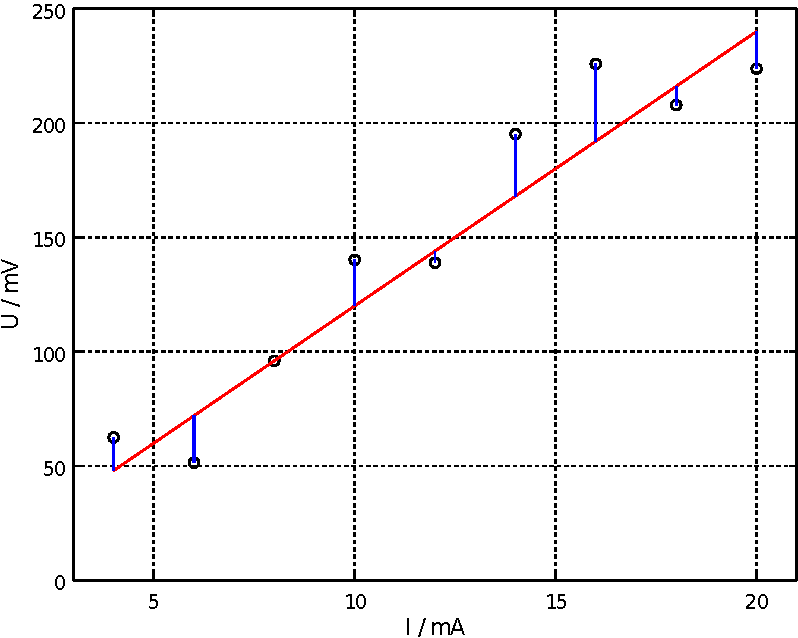
\includegraphics[width=80mm]{01_vorlesung/media/learn_estimation_ohm.pdf}
\caption{Regressionbeispiel: Modellparameter finden, dessen Wert am besten zu den Daten passt}
\label{Ohm1}
\end{center}
\end{figure}

Ob die Spannungswerte zu dem Modell \glqq passen\grqq ~wird bewertet, wobei das Modell
besagt dass die Spannungswerte gleich dem Widerstand, der genau eine konstante Größe sein soll,
multipliziert mit den eingestellten Werten der Stromstärke seien. Das Bewertungskriterium ist
\glqq die Treffer-Wahrscheinlichkeit Spannungswert liegt auf Widerstand mal Strom\grqq.
Wir gehen davon aus, dass die Abweichungen $\varepsilon_i \; = \; U_i \, - \, R I_i$ normalverteilt sind, also
\begin{equation}
p(U_i,I_i | R) \; \propto \; e^{-\frac{1}{2} \left(\frac{\varepsilon_i}{\sigma_\varepsilon}\right)^2}
\end{equation}
wobei $\sigma_\varepsilon$ ein Maß für die Streuung der Residuen, hier in Millivolt, ist.
Wir haben die Werte der Abweichungen $\varepsilon_i$. Man nennt sie \textbf{Residuen}.
Das Produkt aller Wahrscheinlichkeiten $p(U_i,I_i | R)$ heißt \textbf{Likelihood}.
\begin{equation}
L((U_1,\dots, U_J), (I_1,\dots,I_J) | R) \; = \; \prod\limits_{i = 1}^J \, p(U_i,I_i | R)
\end{equation}
Unsere Modellparameter bzw.\ der Modellparameter, die wir ermitteln wollen, ist $R$ und
für die Streuung der Werte des Parameters $R$ verwenden wir das Formelzeichen $\sigma_R$.

In der frequentistischen Statistik wird von der Vorstellung ausgegangen, dass es einen wahren Wert für
$R$ gibt, dem man sich nähert, je mehr und genauer man misst, der aber wegen der Streuung
der Spannungswerte $U$ nur annähernd bestimmbar ist. Wenn wir die Präzisionsstromquelle unverändert
auf einen festen Wert einstellen und nicht durchfahren und dann mehrfach die Spannungen ablesen, so
beobachten wir dennoch leicht unterschiedliche Werte für die Spannung. Dies ist der Grund dafür
dass die Wertepaare bei durchgefahrenem Strom $(I_j, U_j)$ nicht exakt auf einer Geraden liegen.

Am besten passt das ganze für einen Wert für $R$,
für den $L((U_1,\dots, U_J), (I_1,\dots,I_J) | R)$ maximal wird.
Die Zielfunktion unseres Optimierungsvorgangs ist also:
\begin{equation}
\max_{R} \; L((U_1,\dots, U_J), (I_1,\dots,I_J) | R)
\end{equation}
Solch eine Optimierungsaufgabe heißt \textbf{Maximum-Likelihood}-Verfahren.
\begin{equation}
\max_{R} \; \prod\limits_{i = 1}^J \,  e^{-\frac{1}{2} \left(\frac{\varepsilon_i}{\sigma_\varepsilon}\right)^2}
\end{equation}
d.h.\ nach den Gesetzen der Potenzrechnung
\begin{equation}
\max_{R} \; e^{-\frac{1}{2} \sum\limits_{i = 1}^J \, \left(\frac{\varepsilon_i}{\sigma_\varepsilon}\right)^2}
\end{equation}
Das Maximum der Gaußfunktion liegt an der Stelle, an der der Exponent minimal wird.
Wir maximieren die Likelihood, wenn wir ihren Logarithmus minimieren:
\begin{equation}
\min_{R} \; \sum_{i = 1}^J \, \left(\frac{\varepsilon_i}{\sigma_\varepsilon}\right)^2
\end{equation}
dazu suchen wir die Nullstelle der Ableitung nach dem Modellparameter. Hätten wir nicht nur $R$ sondern viele,
dann würden wir den Gradienten bilden.
\begin{equation}
\frac{\partial}{\partial R} \; \sum_{i = 1}^J \, \left(\frac{\varepsilon_i}{\sigma_\varepsilon}\right)^2 \; = \; 0
\end{equation}
d.i.\ in unserem Beispiel
\begin{equation}
\frac{\partial}{\partial R} \; \sum_{i = 1}^J \, \left(\frac{U_i \, - \, R \, I_i}{\sigma_\varepsilon}\right)^2 \; = \; 0
\end{equation}
Wir multiplizieren mit dem Faktor $\sigma_\varepsilon$
\begin{equation}
\frac{\partial}{\partial R} \; \sum_{i = 1}^J \, \left(U_i \, - \, R \, I_i\right)^2 \; = \; 0
\end{equation}
und führen die Differentiation durch
\begin{equation}
\sum_{i = 1}^J \, 2 \left(U_i \, - \, R \, I_i\right) \, I_i \; = \; 0
\end{equation}
Für viele Modellparameter gäbe es entsprechend viele solche Gleichungen mit den jeweiligen Ableitungen, so dass
dann hier ein lineares Gleichungssystem stünde, das zu lösen wäre.
Ein numerisches Verfahren zur Lösung linearer Gleichungssysteme ist das Gauß-Jordan-Eliminationsverfahren.
Nun wir nur diese eine Gleichung haben, können wir einfach nach $R$ auflösen.
\begin{equation}
\sum_{i = 1}^J \, U_i \, I_i \; = \; \sum_{i = 1}^J \, R \, I_i \, I_i
\end{equation}
d.h.
\begin{equation}
 R \; = \; \frac{\sum\limits_{i = 1}^N \, U_i \, I_i}{\sum\limits_{i = 1}^N \,  I_i^2}
\end{equation}
Der ermittelte Wert für $R$ mit den Daten aus der Tabelle ist $12.34~\mathrm{\Omega}$, siehe Abb.~\ref{OhmResult}

\begin{figure}
\begin{center}
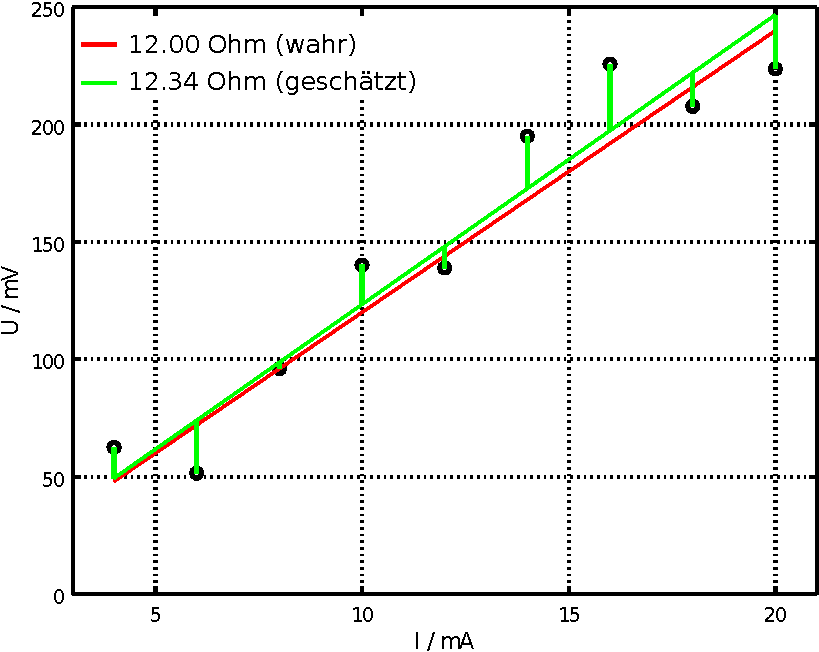
\includegraphics[width=80mm]{01_vorlesung/media/learn_estimation_ohm_esti.pdf}
\label{OhmResult}
\caption{Regressionsbeispiel: Der geschätze Wert des Modellparameters im Vergleich zum wahren.}
\end{center}
\end{figure}

Zuvor haben wir die Likelihood ohne Normierungsfaktor aufgeschrieben.
Eine Wahrscheinlichkeitsdichteverteilung ist so definiert, dass die Fläche unter ihrer Kurve 1 ist, also die Wahrscheinlichkeit
für das Beobachten jedes beliebigen Wertes immer voll eintritt.
\begin{equation}
p(\varepsilon) \; = \; \frac{1}{\sqrt{2 \pi} \sigma_{\varepsilon}} \, e^{-\frac{1}{2} \left(\frac{\varepsilon}{\sigma_{\varepsilon}}\right)^2}
\end{equation}
Ein Maß für die Breite der Gaußglocke ist das $\sigma_{\varepsilon}$ bei etwa 60 Prozent der Höhe ($e^{-\frac{1}{2}} \approx 0.6$).
Ihr Quadrat wird \textbf{Varianz} genannt.
\begin{figure}
\begin{center}
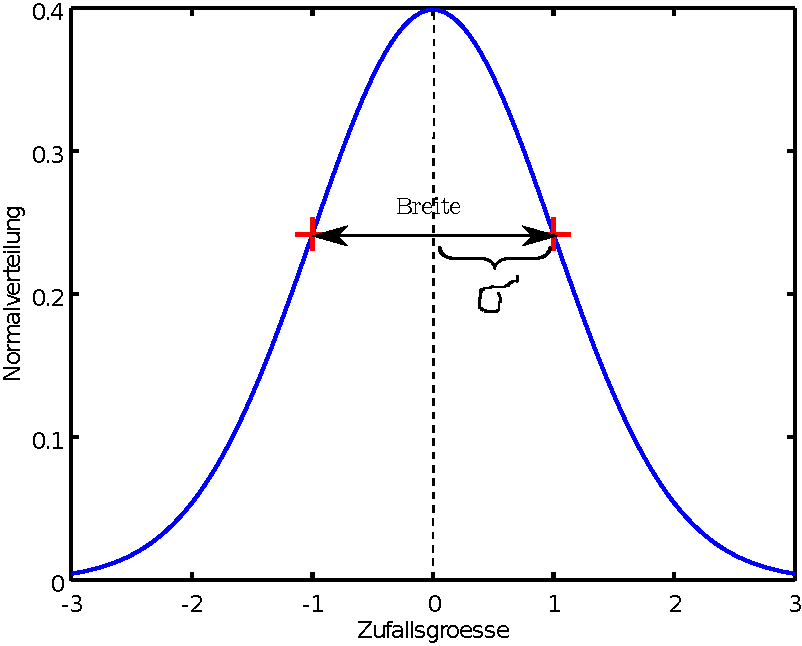
\includegraphics[width=80mm]{01_vorlesung/media/breite_norm_pdf.pdf}
\label{normpdf}
\caption{Breite der Normalverteilung.}
\end{center}
\end{figure}
Das zweite statistische Moment dieser Verteilung 
\begin{equation}
\int_{-\infty}^\infty \, \varepsilon^2 \, p(\varepsilon) \, \mathrm{d} \varepsilon 
\end{equation}
ist gleich dem Quadrat von $\sigma_\varepsilon$, also der Varianz der Gaußverteilung
\begin{equation}
\int_{-\infty}^\infty \, \varepsilon^2 \,  \frac{1}{\sqrt{2 \pi} \sigma_{\varepsilon}} \, e^{-\frac{1}{2} \left(\frac{\varepsilon}{\sigma_\varepsilon}\right)^2} \, \mathrm{d} \varepsilon  \; = \; \sigma_{\varepsilon}^2
\end{equation}
diskretisiert entspricht
\begin{equation}
\frac{1}{\sqrt{2 \pi} \sigma_\varepsilon} \, e^{-\frac{1}{2} \left(\frac{\varepsilon}{\sigma_{\varepsilon}}\right)^2} \, \mathrm{d} \varepsilon
\end{equation}
einer relativen Häufigkeit $\frac{n_k}{J-1}$ in der $k$-ten Klasse der Breite $\mathrm{d} \varepsilon$.
Wenn wir nun kein Histogramm mit gleichgroßen Klassenbreiten bilden, sondern zu jedem $\varepsilon_i$ eine Klasse mit der relativen
Häufigkeit $\frac{1}{J-1}$ betrachten, dann haben wir so ungefähr für das $\sigma_{\varepsilon}^2$
\begin{equation}
\sum_{i=1}^J \, \varepsilon_i^2 \,  \frac{1}{J-1}  \; \approx \; \sigma_{\varepsilon}^2
\end{equation}
Wir nennen diese Breite wegen der Näherung nicht $\sigma_{\varepsilon}^2$. Diese Näherung ist nur ein ungefährer Schätzwert 
und wird \textbf{empirische Varianz} genannt:
\begin{equation}
s_{\varepsilon}^2 \; = \; \frac{1}{J-1} \, \sum_{i=1}^J \, \varepsilon_i^2
\end{equation}
Wir unterscheiden zwischen der Varianz und der empirischen Varianz durch die Verwendung der
unterschiedlichen Formelzeichen $\sigma$ und $s$.

Uns interessiert aber nicht so sehr die Varianz der Residuen $\varepsilon$, die direkt der Varianz
der Spannungsmessung entspricht,
als viel mehr die Varianz des Modellparameters $R$.
Betrachte die Modellgleichung $R \; = \; \frac{U}{I}$, wie empfindlich reagiert die Größe $R$ auf Veränderung der Größe $U$.
Wählt man anstelle eines Wertes $U$ einen Wert $U \, + \, \Delta U$, so reagiert die Größe $R$ über die Modellgleichung wie folgt
\begin{equation}
R \, + \, \Delta R \; = \; \frac{1}{I} \, \left( U \, + \, \Delta U \right)
\end{equation}
d.i. mit $R \; = \; \frac{U}{I}$
\begin{equation}
\Delta R \; = \; \frac{1}{I} \, \left( \Delta U \right)
\end{equation}
Der Differenzenquotient ist also
\begin{equation}
\frac{\Delta R}{\Delta U} \; = \; \frac{1}{I}
\end{equation}
was bei diesem linearen Zusammenhang direkt hinkommt. Allgemein passt es für stetige Modelle auch bei nichtlinearem Zusammenhang
für genügend kleine Änderungen. Deshalb wird die Empfindlichkeit, die \textbf{Sensitivität}, definiert
\begin{equation}
c  \; = \; \frac{\partial R}{\partial U}
\end{equation}
Die Varianz ist eine quadratische Veränderung, so dass
\begin{equation}
s_R^2  \; = \; \left(\frac{\partial R}{\partial U}\right)^2 \, s_{\varepsilon}^2 \; = \; \frac{1}{I^2} \, s_{\varepsilon}^2
\end{equation}
Hier hätte ich auch direkt $s_R$ aufschreiben können, aber die quadratische Schreibweise wird erforderlich, wenn es um mehrere Größen geht. In den folgenden Vorlesungen werden wir das Konzept der Fortpflanzung der Varianzen kennen lernen.

Die Varianzen sind ein Maß für die Unsicherheit von Messungen. Die \textbf{Messunsicherheit} ist zentrales Thema in der Messtechnik.
\begin{quote}
\textbf{Messunsicherheit; Unsicherheit} (engl. \textsl{measurement uncertainty; uncertainty}): 
nichtnegativer Parameter, der die Streuung der Werte kennzeichnet, die der Messgröße
auf der Grundlage der benutzten Information beigeordnet ist. [VIM2.26]
\end{quote}
Sie drückt den Mangel einer genauen Kenntnis des Wertes der Messgröße aus.
Selbst wenn systematische Effekte korrigiert werden, bleibt der \textbf{Messwert} lediglich
ein \textbf{Schätz\-wert der Messgröße}, siehe auch GUM:2008, Abschnitt 3.3.1 .

Im Bereich der Metrologie wird zum Thema Messunsicherheitsberechnung eine Richtlinie verwendet,
um die Auswerteverfahren im gesetzlichen Messwesen zu vereinheitlichen und die Resultate
besser vergleichbar zu machen. Die Richtlinie wurde von der
\textsl{Working Group} 1 des \textsl{Joint Committee for Guides in Metrology} (JCGM/WG 1)
entwickelt. Sie hat den Titel \textsl{Evaluation of measurement
data - Guide to the expression of uncertainty in measurement} und wird mit GUM abgekürzt.
Die derzeit gültige Version ist
\textsl{JCGM 100:2008 GUM 1995 with minor corrections} und ist in englischer Fassung
auf der Webseite des \textsl{Bureau international des poids et mesures} (BIPM)
unter folgendem Link frei erhältlich:
\begin{verbatim}
https://www.bipm.org/utils/common/documents/jcgm/JCGM_100_2008_E.pdf
\end{verbatim}

In vielen Fällen reicht es, die Varianzen der einzelnen direkten Messgrößen zu untersuchen sowie
den Zusammenhang zwischen der Variation einer direkten Messgröße und die dadurch verusachte
Veränderung der indirekten. Dieser Zusammenhang ist zentrales Thema der Bestimmung von Messunsicherheiten
und wird im Laufe dieser Vorlesung eingehend beleuchtet.
Vielfach gibt es nicht nur einen Zusammenhang zwischen einer direkten mit einer indirekten Messgröße,
sondern auch einen Zusammenhang zwischen den direkten Messgrößen untereinander.

In dieser Vorlesungsreihe liegt das Hauptaugenmerk auf linearen Zusammenhängen zwischen Messgrößen,
zum einen zwischen den direkten untereinander und zum anderen zwischen der indirekten mit den jeweiligen
direkten. Die lineare Beziehung zwischen den direkten Größen untereindander wird für die Unsicherheitsfortpflanzung
sowie für die lineare Regression benötigt. Das Maß für den linearen Zusammenhang wird \textbf{Korrelation} genannt.
Bei der linearen Regression geht es um Modelle mit indirekten Messgrößen,
die als Koeffizienten eines Polynoms auftreten. Um den Grad des Polynoms zu ermitteln, wird untersucht bis
mit welchem Potenzgesetz ein paar direkter Messgrößen zu verknüpfen ist (welchen Grad das Polynom hat),
so dass die Korrelation groß ist.


\section{Charakterisierung von linearem Zusammenhang zwischen Größen}


Bei dem Beispiel mit dem Ohm'schen Gesetz hatten wir uns auch mit der Modellgleichung $U = R I$ befasst.
Dabei waren $U$ und $I$ die beiden physikalischen Größen, die unterschiedliche Werte angenommen haben und
einen linearen Zusammenhang. Hier haben wir also eine Gerade, Polynom vom Grad 1.

Für eine Bewertung von Wechselwirkungen zwischen Effekten werden in der Statistik Maße
definiert, die die Stärke und eventuell auch Richtung eines Zusammenhangs zwischen dem
Auftreten zufälliger Ereignisse quantifizieren sollen. Wir hatten das Beispiel des Ohm'schen
Gesetzes betrachtet, bei dem es einen Zusammenhang zwischen Stromstärke und elektrischer
Spannung gibt. Der Zusammenhang ist in diesem Beispiel ein linearer.

Für die Charakterisierung \textsl{linearer} Zusammenhänge ist der
\textbf{Korrelationskoeffizient} $\rho$ ein Maß, mit dem quantifiziert wird, wie
stark zwei Größen linear miteinander verknüpft sind.
Der Korrelationskoeffizient ist definiert, dass er Werte zwischen $-1$ und
$1$ annehmen kann. Gibt es einen direkten linearen Zusammenhang zwischen zwei Zufallsgrößen
$X_1$ und $X_2$, so wird man zu einer Beobachtung der einen Größe mit kleinem Wert
auch einen kleinen Wert bei der anderen Größe beobachten und wenn die eine Größe einen
großen Wert annimmt, so wird die andere auch einen großen Wert annehmen, und
$\rho$ wird in der Nähe von $1$ liegen. Haben zwei Zufallsgrößen einen ebenso
direkten Zusammenhang, aber in umgekehrter Weise, dass zu kleinen Werten von der ersten
Größe große Werte zur zweiten Größe auftreten und umgekehrt, so liegt $\rho$ in der Nähe von $-1$.
In beiden Fällen sagt man, dass die Größen \textbf{korreliert} seien.

Gibt es überhaupt gar keinen Zusammenhang zwischen dem, was an Werten zu der einen Größe beobachtet
wird mit dem, was an Werten zu der anderen Größe beobachtet wird, so ist $\rho = 0$ und man
sagt die beiden Größen seien \textbf{unkorreliert}.

\begin{figure}
	\begin{center}
		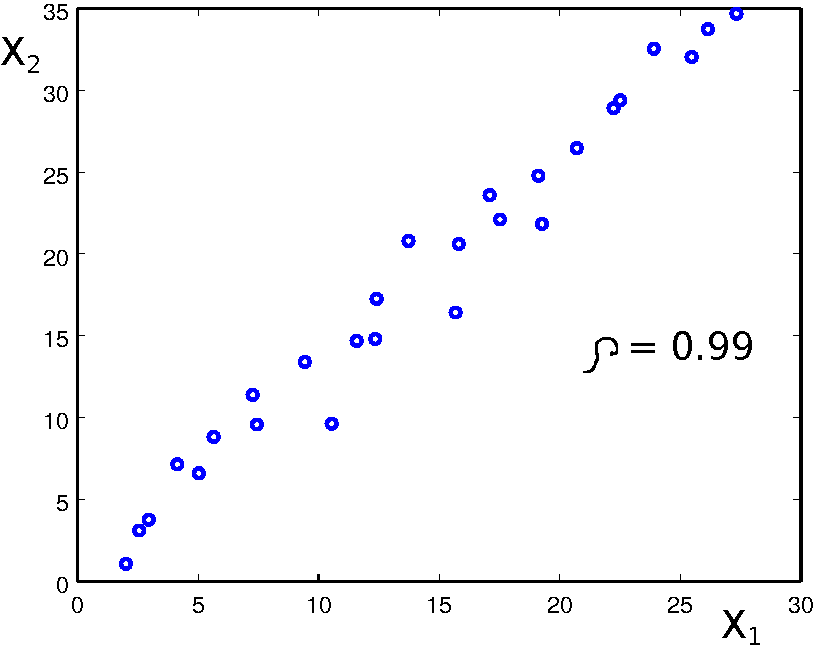
\includegraphics[width=75mm]{01_vorlesung/media/korreliert.pdf} \hspace{5mm}
		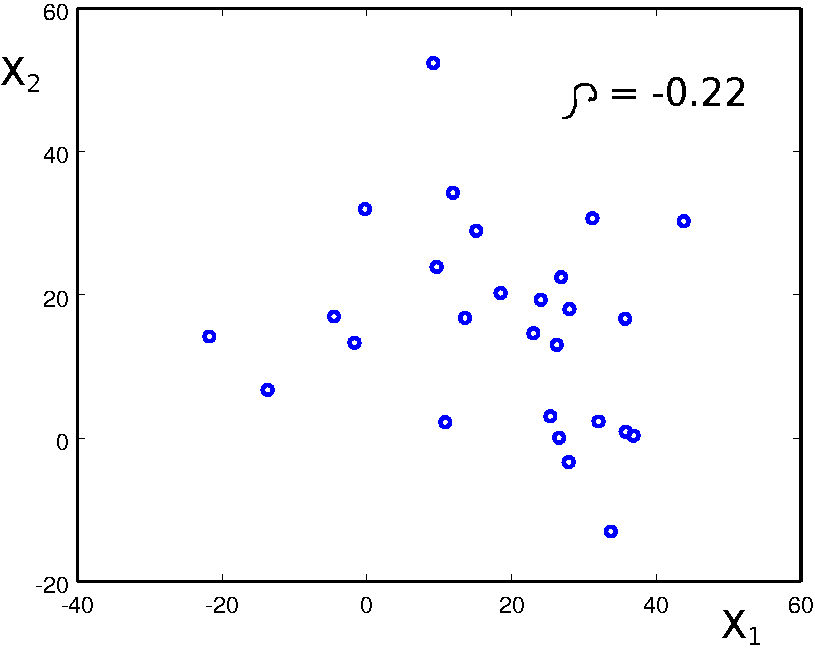
\includegraphics[width=75mm]{01_vorlesung/media/unkorreliert.pdf}
		\caption{\label{korrelation} Wenn es einen linearen Zusammenhang zwischen
			zwei Zufallsgrößen $X_1$ und $X_2$ gibt, so sagt man, dass sie korreliert sind
			und der Korrelationskoeffizient $\rho$ liegt bei Eins (\textsl{links}) oder bei
			minus Eins. Wenn es keinen Zusammenhang zwischen zwei Zufallsgrößen $X_1$ und $X_2$
			gibt, so sagt man, dass sie unkorreliert sind
			und der Korrelationskoeffizient $\rho$ liegt bei Null (\textsl{rechts}).}
	\end{center}
\end{figure}

Die Erwartungswerte zu jeder der Größen $X_1$ und $X_2$ sind jeweils
$\mathrm{E}(X_1)$ und $\mathrm{E}(X_2)$. Sie werden aus den Mittelwerten der jeweiligen
Stichproben geschätzt
\begin{equation}
\bar x_1 \; = \; \frac{1}{J} \, \sum_{j = 1}^J X_{1,j} \qquad
\bar x_2 \; = \; \frac{1}{J} \, \sum_{j = 1}^J X_{2,j}
\end{equation}
Dann ist
\begin{equation}
\mathrm{\bar X} \; = \;
\left(\begin{array}{c}
\bar x_1 \\
\bar x_2
\end{array}
\right)
\end{equation}
der Schwerpunkt der Beobachtungen der Größen.
Sind die Entfernungen der Beobachtungs\-pärchen $(X_{1,j}, X_{2,j})$ vom Schwerpunkt so,
dass die Richtungskomponente der Größe $X_1$ in die gleiche Richtung weist und auch in
proportionale Entfernung wie die Richtungskomponente der Größe $X_2$, so liefern die 
Produkte $(X_{1,j} - \bar x_1)(X_{2,j} - \bar x_2)$ gleiche Vorzeichen. Streuen diese
aber unzusammenhängend, so mitteln sich die unterschiedlichen Terme
$(X_{1,j} - \bar x_1)(X_{2,j} - \bar x_2)$ bei Summation weg.

Wir definieren die Größe
\begin{equation}
s_{1,2} \; := \; \frac{1}{J-1} \, \sum_{j = 1}^J (X_{1,j} - \bar x_1)(X_{2,j} - \bar x_2)
\end{equation}
und nennen sie die \textbf{empirische Kovarianz}.
Allgemein ist die \textbf{Kovarianz} für Zufallsgrößen, deren gemeinsame Verteilung
ihre Wahrscheinlichkeitsdichte $p(X_1, X_2)$ sei, wie folgt definiert
\begin{equation}
\operatorname{Cov}(X_1, X_2) \; := \; 
\int\limits_{-\infty}^{\infty}\int\limits_{-\infty}^{\infty}
(X_1^\prime \, - \operatorname{E}(X_1))(X_2^\prime \, - \operatorname{E}(X_2)) \,
p(X_1^\prime, X_2^\prime) \, \operatorname{d} X_1^\prime \operatorname{d} X_2^\prime .
\end{equation}
Wir sehen hier, dass die Kovarianz einer Zufallsgröße mit sich selbst die
\textbf{Varianz} ist
\begin{equation}
\operatorname{Var}(X_1) \; := \;  \operatorname{Cov}(X_1, X_1) \; = \; 
\int\limits_{-\infty}^{\infty}
(X_1^\prime \, - \operatorname{E}(X_1))^2 \,
p(X_1^\prime) \, \operatorname{d} X_1^\prime
\end{equation}
und für die empirsche Varianz und Kovarianz gilt entsprechend
\begin{equation}
s_{1}^2 \; := \; s_{1,1} \; = \; 
\frac{1}{J-1} \, \sum_{j = 1}^J (X_{1,j} - \bar x_1)^2 .
\end{equation}
Wir haben bereits in der 2. Vorlesung gesehen, dass bei der Steigung der Regressionsgraden
(Aufgabe 1) genau so ein Term $\sum_{j = 1}^J (X_{1,j} - \bar x_1)(X_{2,j} - \bar x_2)$
im Zähler steht.

Für das Verständnis der Gesamtzusammenhänge ist der Sprachgebrauch für Zufallsgrößen sowie
der Sprachgebrauch des Erwartungswertes von Zufallgrößen von Bedeutung. 

Verknüpfungen von Zufallsgrößen sind ihrerseits wieder Zufallsgrößen. Betrachten
wir eine Größe $X$, die ganz abstrakt und allgemein eine Zufallsgröße ist, und
$p(X)$ die Wahrscheinlichkeitsdichteverteilung dazu, so heißt
\begin{equation}
\operatorname{E}(X) \; := \;  \int\limits_{-\infty}^{\infty}
X^\prime \, p(X^\prime) \, \operatorname{d} X^\prime
\end{equation}
Erwartungswert der Zufallsgröße $X$.
Ist diese Zufallsgröße eine Verknüpfung von anderen Zufallsgrößen und setzen wir die
Verknüpfung ein, so wird der Erwartungwert mit derselben Verknüpfung gebildet.
Betrachten wir zum Beispiel die Verknüpfung Addition $X = X_1 + X_2$
\begin{equation}
\operatorname{E}(X_1 + X_2) \; := \;  \int\limits_{-\infty}^{\infty} \int\limits_{-\infty}^{\infty}
(X_1^\prime + X_2^\prime) \, p(X_1^\prime, X_2^\prime) \, \operatorname{d} X_1^\prime \, \operatorname{d} X_2^\prime
\end{equation}
d.h.
\begin{equation}
\arraycolsep=2.0pt\def\arraystretch{2.0}
\begin{array}{ll}
\operatorname{E}(X_1 + X_2) \; = & \int\limits_{-\infty}^{\infty} \int\limits_{-\infty}^{\infty}
X_1^\prime \, p(X_1^\prime, X_2^\prime) \, 
\operatorname{d} X_1^\prime \, \operatorname{d} X_2^\prime\\
& + \; \int\limits_{-\infty}^{\infty} \int\limits_{-\infty}^{\infty} 
X_2^\prime \, p(X_1^\prime, X_2^\prime) \, \operatorname{d} X_1^\prime \, \operatorname{d} X_2^\prime
\end{array}
\end{equation}
und mit der Randverteilung (engl.\ \textsl{marginal distribution}) 
\begin{equation}
p(X_2) \; = \;
\int\limits_{-\infty}^{\infty} p(X_1^\prime, X_2) \, \operatorname{d} X_1^\prime
\label{marginalDistr}
\end{equation}
erhalten wir
\begin{equation}
\operatorname{E}(X_1 + X_2) \; = \; \int\limits_{-\infty}^{\infty}
X_1^\prime \, p(X_1^\prime) \, \operatorname{d} X_1^\prime 
\; + \; \int\limits_{-\infty}^{\infty} 
X_2^\prime \, p(X_2^\prime) \, \operatorname{d} X_2^\prime
\end{equation}
also
\begin{equation}
\operatorname{E}(X_1 + X_2) \; = \; \operatorname{E}(X_1) \; + \; \operatorname{E}(X_2).
\label{EwSummeISTSummeEw}
\end{equation}
In Worten heißt dies: Der Erwartungswert einer Summe von Zufallsgrößen ist die
Summe der Erwartungswerte der Zufallsgrößen.

Als nächstes betrachten wir das Produkt zweier Zufallsgrößen
$X = X_1 \cdot X_2$
\begin{equation}
\operatorname{E}(X_1 \cdot X_2) \; := \; 
\int\limits_{-\infty}^{\infty} \int\limits_{-\infty}^{\infty}
X_1^\prime \, X_2^\prime \; p(X_1^\prime, X_2^\prime) \,
\operatorname{d} X_2^\prime\, \operatorname{d} X_1^\prime .
\end{equation}
Die Kovarianz ist der Erwartungswert folgenden Produktes
$(X_1 - \operatorname{E}(X_1)) \cdot (X_2 - \operatorname{E}(X_2))$
\begin{equation}
\operatorname{E}((X_1 - \operatorname{E}(X_1)) \cdot
(X_2 - \operatorname{E}(X_2))) \; = \; 
\int\limits_{-\infty}^{\infty} \int\limits_{-\infty}^{\infty}
(X_1^\prime - \operatorname{E}(X_1)) \cdot (X_2^\prime - \operatorname{E}(X_2))
\, p(X_1^\prime, X_2^\prime) \, 
\operatorname{d} X_1^\prime\, \operatorname{d} X_2^\prime
\end{equation}
also
\begin{equation}
\operatorname{Cov}(X_1, X_2)  \; = \; \operatorname{E}\left((X_1 - \operatorname{E}(X_1)) 
\cdot (X_2 - E(X_2)) \right)  .
\end{equation}
Ferner ist zu bemerken, dass sich aus diesen Beziehungen für die
Kovarianz ergibt
\begin{equation}
\begin{array}{ll}
\operatorname{Cov}(X_1, X_2)
& \; = \;  \operatorname{E}\left(X_1 \, X_2 - X_2 \, \operatorname{E}(X_1) -
X_1 \, \operatorname{E}(X_2) + \operatorname{E}(X_1) \, \operatorname{E}(X_2) \right) \\
& \; = \;  \operatorname{E}(X_1 \, X_2)  - \operatorname{E}(X_2) \, \operatorname{E}(X_1)
- \operatorname{E}(X_1) \, \operatorname{E}(X_2) + \operatorname{E}(X_1) \, \operatorname{E}(X_2)) \\
& \; = \;  \operatorname{E}(X_1 \, X_2) - \operatorname{E}(X_1) \, \operatorname{E}(X_2) .
\end{array}
\label{ErwartungsCOV}
\end{equation}
Per Definitionem gilt
\begin{equation}
\operatorname {Var}(X) \; := \; \operatorname {Cov}(X,X) .
\end{equation}
Daraus folgt, dass für die Varianz einer Zufallsgröße,
die das Produkt einer Zufallsgröße $X$ mit einem konstanten, festen reellen Faktor $b$ ist, gilt
\begin{equation}
\operatorname {Var}(b X) \; := \; b^2 \, \operatorname {Var}(X)
\end{equation}
%Für einen Zufallsgrößenvektor $\boldsymbol{X}$ multipliziert mit einer Matrix 
%$\boldsymbol{B}$, deren Elemente konstante, feste reelle Zahlen sind, gilt entsprechend
%\begin{equation}
%\operatorname {Cov}(\boldsymbol{B} \boldsymbol{X}) \; := \; \boldsymbol{B} \,
% \operatorname {Cov}(\boldsymbol{X}) \, \boldsymbol{B}^\mathsf{T} .
%\label{CovarianzKonstMatrix}
%\end{equation}
%Das ist jetzt nicht trivial herzuleiten, aber wir wollen jetzt keine Vorlesung in Lineare
%Algebra halten. Wir werden diese Beziehung für die Bestimmung der Standardabweichung der
%Modellparameter in der linearen Regression brauchen. Das hochgestellte $\mathsf{T}$ steht für
%transponiert.

Eine weitere wichtige Beziehung ist folgende zur
\textbf{Varianz einer Summe von Zufallsgrößen}:
\begin{equation}
\operatorname {Var}\left(\sum _{{i=1}}^{N}X_{i}\right) \; = \;
\sum _{{i,j=1}}^{N}\operatorname {Cov}(X_{i},X_{j})
\label{VarianzSummeISTSummeKovarianz}
\end{equation}
Die Varianz ist nach Definition
\begin{equation}
\operatorname {Var}\left(\sum _{{i=1}}^{N}X_{i}\right) \; = \;
\int\limits_{-\infty}^{\infty} \dots \int\limits_{-\infty}^{\infty}
\, \left[ \left(\sum_{i=1}^N X_i\right) \; - \; E(\sum_{i=1}^N X_i) \right]^2 \, p(X_1, \dots, X_2)
\, \operatorname{d}X_1 \dots \operatorname{d}X_N .
\end{equation}
Da der Erwartungswert einer Summe von Zufallsgrößen gleich der Summe der 
Erwartungswerte jeder einzelnen dieser Zufallsgrößen ist, siehe Gl.~(\ref{EwSummeISTSummeEw}), gilt
$$
\left(\sum_{i=1}^N X_i \right) \; - \; E(\sum_{i=1}^N X_i) \; = \;
\left(\sum_{i=1}^N X_i \right) \; - \; \sum_{i=1}^N E(X_i) 
$$
so dass gilt
\begin{equation}
\operatorname {Var}\left(\sum _{{i=1}}^{N}X_{i}\right) \; = \;
\int\limits_{-\infty}^{\infty} \dots \int\limits_{-\infty}^{\infty}
\, \left[ \sum_{i=1}^N \left(X_i \; - \; E(X_i)\right) \right]^2 \, p(X_1, \dots, X_2)
\, \operatorname{d}X_1 \dots \operatorname{d}X_N .
\end{equation}
Mit Anwendung des Assoziativgesetzes
$$
\arraycolsep=3.5pt\def\arraystretch{1.8}
\begin{array}{ll}
\left[ \sum\limits_{i=1}^N \left(X_i \; - \; E(X_i)\right) \right]^2 & =
\left[ \sum\limits_{i=1}^N \left(X_i \; - \; E(X_i)\right) \right] \;
\left[ \sum\limits_{k=1}^N \left(X_k \; - \; E(X_k)\right) \right] \\
& = \sum\limits_{i=1}^N \sum\limits_{k=1}^N  \left(X_i \; - \; E(X_i)\right) \;
\left(X_k \; - \; E(X_k)\right) \\
\end{array}
$$
gilt
\begin{equation}
\operatorname {Var}\left(\sum _{{i=1}}^{N}X_{i}\right) \; = \;
\int\limits_{-\infty}^{\infty} \dots \int\limits_{-\infty}^{\infty}
\, \sum_{i=1}^N \sum_{k=1}^N  \left(X_i \; - \; E(X_i)\right) \;
\left(X_k \; - \; E(X_k)\right) \, p(X_1, \dots, X_2)
\, \operatorname{d}X_1 \dots \operatorname{d}X_N .
\end{equation}
Durch Berechnung der Marginalverteilungen und weil $\int p(X_j) \, \operatorname{d}X_j = 1$
für alle $j$, die weder $i$ noch $k$ sind, erhalten wir
\begin{equation}
\operatorname {Var}\left(\sum _{{i=1}}^{N}X_{i}\right) \; = \;
\sum_{i=1}^N \sum_{k=1}^N  \;
\int\limits_{-\infty}^{\infty} \int\limits_{-\infty}^{\infty}
\, \left(X_i \; - \; E(X_i)\right) \;
\left(X_k \; - \; E(X_k)\right) \, p(X_i, X_k)
\, \operatorname{d}X_i \operatorname{d}X_k .
\end{equation}
Der Term auf der rechten Seite ist genau die Kovarianz der beiden 
Größen $X_i$ und $X_k$.

Die Beziehung Gl.~(\ref{VarianzSummeISTSummeKovarianz}), dass die
Varianz der Summe von Zufallsgrößen gleich der Summe der paarweisen Kovarianzen
ist, werden wir im Laufe dieser Vorlesungsreihe häufig
verwenden:
\begin{equation}
{\begin{aligned}\operatorname {Var}\left(\sum _{{i=1}}^{N}X_{i}\right) & 
	= \sum _{i=1}^{N}\sum _{k=1}^{N}\operatorname {Cov}(X_{i},X_{k})\\
	& = \sum _{{i=1}}^{N}\operatorname {Var}(X_{i})+
	\sum _{{i,k=1,i\neq k}}^{N}\operatorname {Cov}(X_{i},X_{k})\\
	& = \sum _{i=1}^{N}\operatorname {Var}(X_{i})+2\sum _{{i=1}}^{{N-1}}
	\sum _{k=i+1}^{N}\operatorname {Cov}(X_{i},X_{k}) ,
	\end{aligned}}
\label{VarianzSummeX2Kovarianz}
\end{equation}
Dies lässt sich für den Fall erweitern, dass die summierten Zufallsgrößen mit jeweils einem reellen,
konstanten Faktor multipliziert werden:
\begin{equation}
{\begin{aligned}\operatorname {Var}\left(\sum _{{i=1}}^{N} \, c_i \, X_{i}\right) & 
	= \sum _{i=1}^{N}\sum _{k=1}^{N}\operatorname {Cov}(c_i X_{i}, c_k X_{k})\\
	& = \sum _{{i=1}}^{N} \, c_i^2 \, \operatorname {Var}(X_{i})+
	\sum _{{i,k=1,i\neq k}}^{N} \, c_i c_k \,  \operatorname {Cov}(X_{i},X_{k})\\
	& = \sum _{{i=1}}^{N} \, c_i^2 \operatorname {Var}(X_{i})+2\sum _{{i=1}}^{{N-1}}
	\sum _{{k=i+1}}^{N} \, c_i c_k \operatorname {Cov}(X_{i},X_{k}).
	\end{aligned}}
\label{KovarianzSumme}
\end{equation}
Auf Gleichung (\ref{KovarianzSumme}) werden wir in den nächsten Vorlesungen zurück kommen,
denn diese ist die Grundlage für das \textbf{Gesetz zur Fortpflanzung von Messunsicherheiten}.

Für standardnormalverteilte Zufallsgrößen $Z_i$ mit $Z \sim \mathcal{N}(0,1)$ 
und $i = 1,2$ in die sich
die Größen $X_i$ wie folgt umrechnen lassen
\begin{equation}
Z_i \; = \; \frac{X_i \, - \, \operatorname{E}(X_i)}{\sqrt{\operatorname {Var}(X_{i})}}
\end{equation}
ist die Kovarianz gleich dem Korrelationskoeffizienten
\begin{equation}
\rho_{i,k} \; = \; \operatorname {Cov}(Z_{i},Z_{k})
\end{equation}
was äquivalent ist zu
\begin{equation}
\rho_{i,k} \; = \; \frac{\operatorname {Cov}(X_{i},X_{k})}{\sqrt{\operatorname {Var}(X_{i})} \, \sqrt{\operatorname {Var}(X_{k})}} .
\end{equation}


\section{Beispiel zum Selbststudium}
Zu Bestimmen ist ein Ohmscher Widerstand $R$ sowie eine Offsetspannung $U_0$ bei gegebenen Werten einer
Präzisionsstromquelle und eines Voltmeters:

\begin{center}
\begin{tabular}{l||c|c|c|c|c|c|c|c|c}
\hline\hline
 $I$ in mA &    4.0 &     6.0 &     8.0 &    10.0 &    12.0 &    14.0 &    16.0 &    18.0 &    20.0\\
\hline
 $U$ in mV &    62.5 &    51.5 &    96.0 &   140.2 &   138.9 &   195.1 &   225.8 &   207.8 &   223.7 \\
\hline\hline
\end{tabular}
\end{center}

Es wird angenommen, dass die Stromstärken ohne Streuung vorliegen (als Regressoren) und die Spannungen normalverteilt
streuen (als Regressanden), so dass
\begin{equation}
\min_{R, U_0} \; \sum_{i = 1}^J \, \left(U_i \, - \, R \, I_i  \, - \,  U_0\right)^2
\label{regrGer}
\end{equation}

\begin{itemize}
\item[(a)] Berechnen Sie den Korrelationskoeffizienten $\rho(I, U)$
\item[(b)] Lösen Sie das Gleichungssystem
\begin{equation}
\left(\begin{array}{c}
\frac{\partial}{\partial R}\\
\frac{\partial}{\partial U_0}
\end{array}\right)
\, \sum_{i = 1}^J \, \left(U_i \, - \, R \, I_i  \, - \,  U_0\right)^2 \; = \;
\left(\begin{array}{c}
0\\
0
\end{array}\right)
\label{regrGerGS}
\end{equation}
\item[(c)] Berechnen Sie die aus der Lösung des Gleichungssystems aus (a) gewonnen Schätzwerte
für $R$ und $U_0$.
\end{itemize}



